\documentclass{beamer}
\usepackage[utf8]{inputenc}
\usetheme{Antibes}
\usepackage{color}

\title{- Soutenance -\\ Conception d'un Tetris}
\author{\textsc{André} Lorada  (21809742) \\ \textsc{Lebranchu} Paul  (21403460) \\ \textsc{Levesque} Willy  (21808901)  \\ \textsc{Lopez-pardo} Hugues  (21803489) }
\institute{Université de Caen Normandie}


\begin{document}

\begin{frame}
	\begin{figure}[t]
        
\includegraphics[scale=0.75]{images/logo.png}
	\end{figure}
	
	\titlepage
\end{frame}


\begin{frame}
	\tableofcontents
\end{frame}

\section{Introduction}

	\begin{frame}
	    \begin{center}
	        
\includegraphics[scale=0.1]{images/logoTetris.png}
	    \end{center}
	    \begin{itemize}
	        \item Objectif: concevoir un jeu Tetris en python, avec la bibliothèque Pygame.
	        \item D'après Wikipédia, le Tetris est "un jeu vidéo de puzzle conçu par Alekseï Pajitnov à partir de juin 1984 ".
	        \item Fonctionnalités: Tetris basique, mode multijoueurs.
	    \end{itemize}
	\end{frame}
	
	
\section{Gestion des écrans du menu}
	
	\begin{frame}{Pourquoi une gestion des écrans?}
    
    	\begin{itemize}
    	    \item plusieurs écrans dans le jeu
    	    \newline
    	    
    	    \item meilleure lisibilité du code
    	    \newline
    	    
    	    \item meilleure organisation
    	\end{itemize}
	\end{frame}
    
    
    \begin{frame}{Structure}
        \begin{figure}
            \centering
            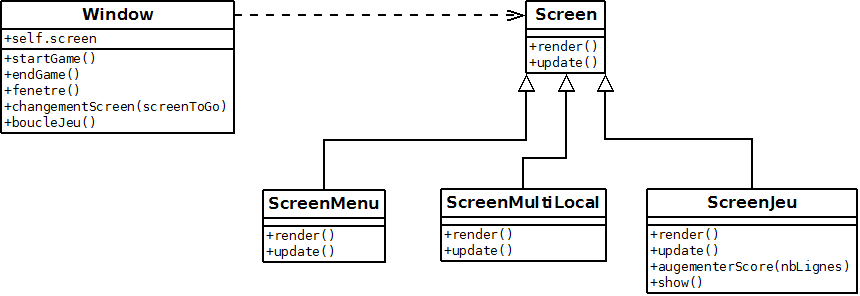
\includegraphics[scale=0.37]{images/dia.png}
        \end{figure}
    \end{frame}
    
    
    \begin{frame}{Le passage d'un écran à l'autre}
        \begin{figure}
            \centering
             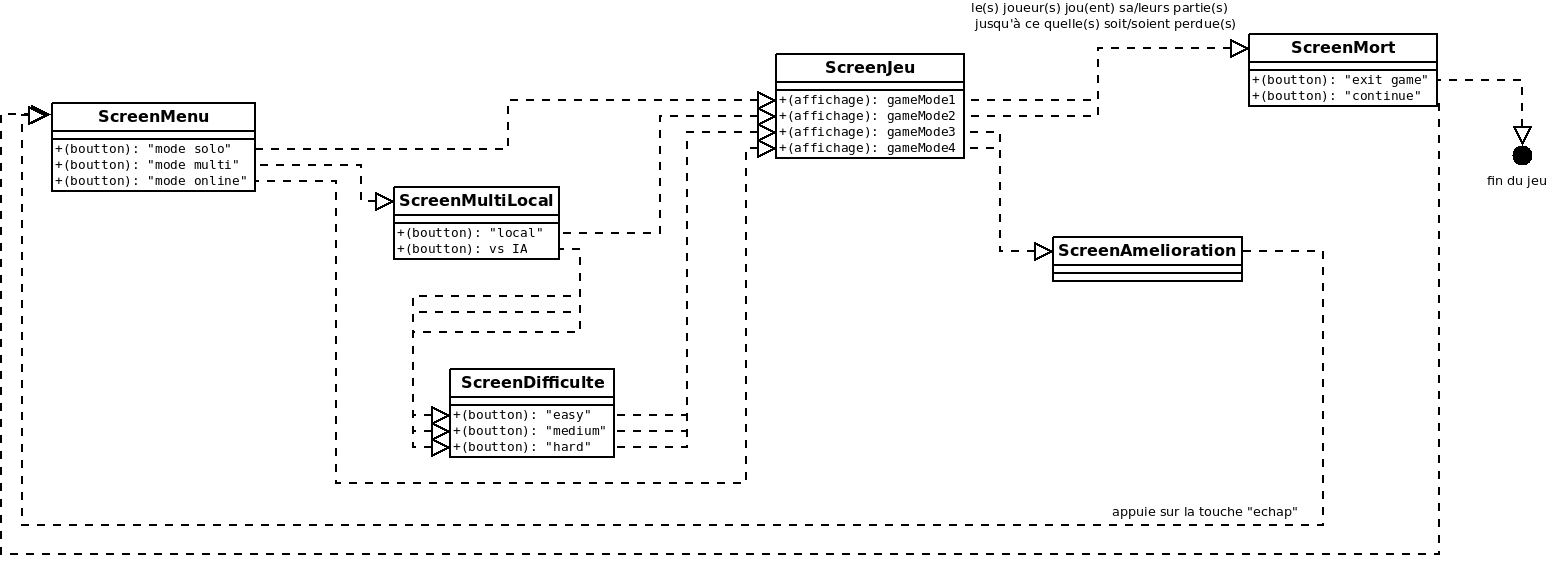
\includegraphics[scale=0.15]{images/diagrammeEvenementiel.png}
        \end{figure}
        
        \begin{figure}
            \centering
             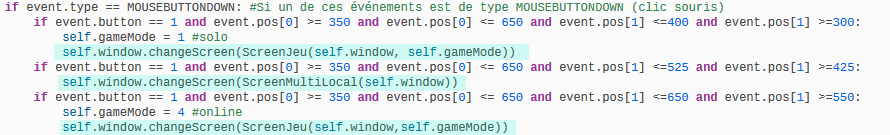
\includegraphics[scale=0.45]{images/changementEcran.png}
        \end{figure}
        
         \begin{figure}
            \centering
            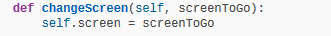
\includegraphics[scale=0.5]{images/fonctChangScreen.png}
        \end{figure}
    \end{frame}

\section{Explication des mécanismes du jeu}
	
	
	\begin{frame}{Création et affichage de la grille}
		Création d'un tableau puis affichage du contenu du tableau:
		
		\begin{figure}[t]
		
        	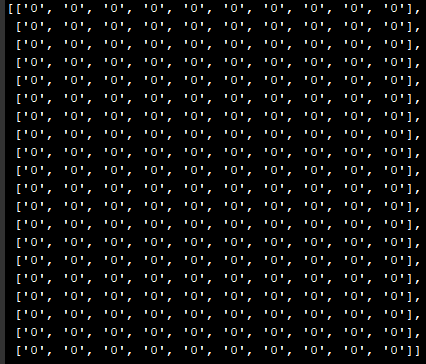
\includegraphics[scale=0.45]{images/tableau_de_la_grille.PNG}\hfill      	
        	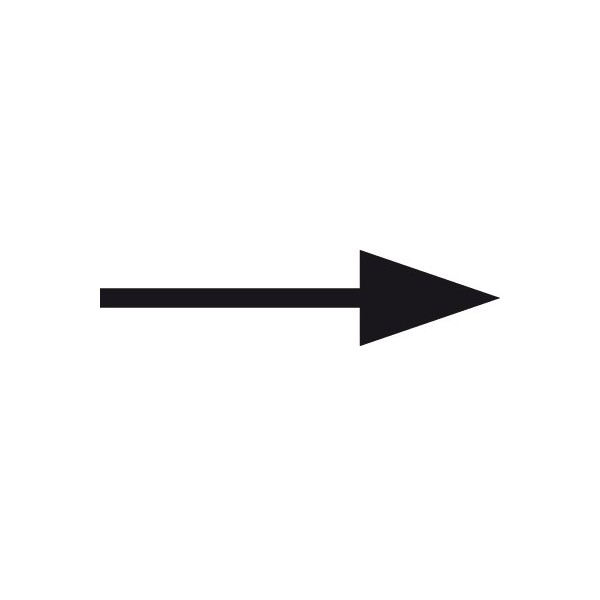
\includegraphics[scale=0.07]{images/image.jpg} \hfill        	
        	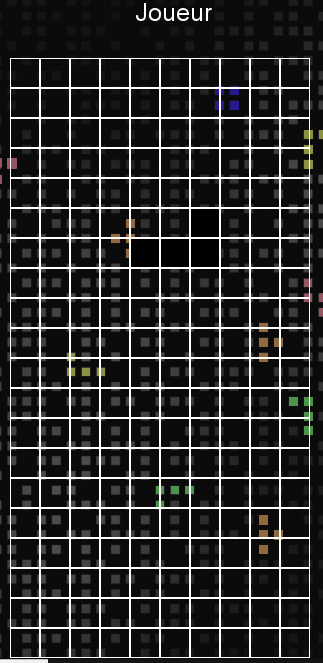
\includegraphics[scale=0.25]{images/grille_afficher.PNG}
        	
		\end{figure}
		
	\end{frame}
	
	
	\begin{frame}{Gestion de la chute des pièces et des déplacements}
	
		\begin{enumerate}
		
			\item Sélection des pièces
			
			\begin{figure}[t]
			
        	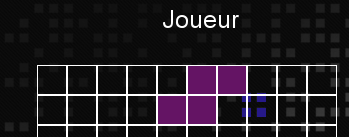
\includegraphics[scale=0.4]{images/Piece.PNG}\hfill
        	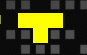
\includegraphics[scale=0.5]{images/piece_suivante.PNG}
        	
			\end{figure}
			
			\item Déplacement vers la gauche, vers la droite, vers le bas et chute automatique
			\newline
			
			\item Rotation des pièces
			\begin{figure}[t]
			
        	
\includegraphics[scale=0.6]{images/exe.PNG}\hfill
        	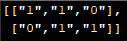
\includegraphics[scale=0.6]{images/exeConsole.PNG}\hfill
        	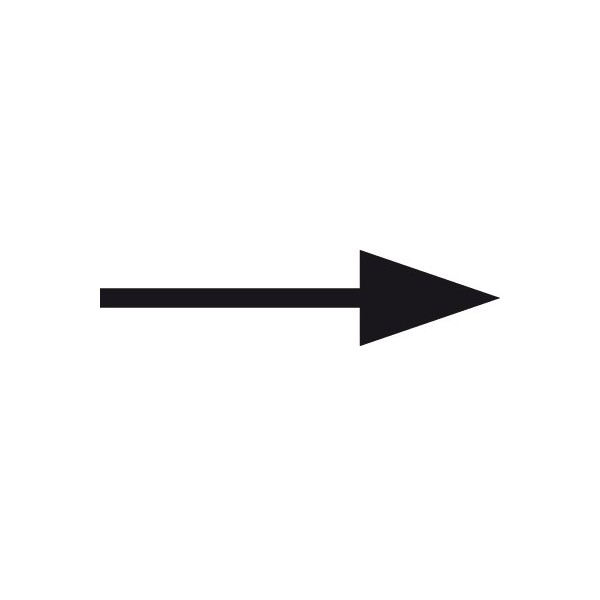
\includegraphics[scale=0.04]{images/image.jpg} \hfill 
        	
\includegraphics[scale=0.6]{images/rotat.PNG}
        	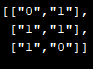
\includegraphics[scale=0.6]{images/rotatConsole.PNG}\hfill
        	
			\end{figure}.
			
		\end{enumerate}
			
	
	\end{frame}
	
	
	\begin{frame}{Gestion des collisions,du score et des niveaux}
	
		\begin{enumerate}
			\item Gestion de la collision des pièces (pygame: collidelistall)
			\newline
			
			\item Implémentation des pièces dans la grille
			\newline
			
			\begin{figure}[t]
			
        	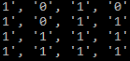
\includegraphics[scale=0.8]{images/console.PNG}\hfill
        	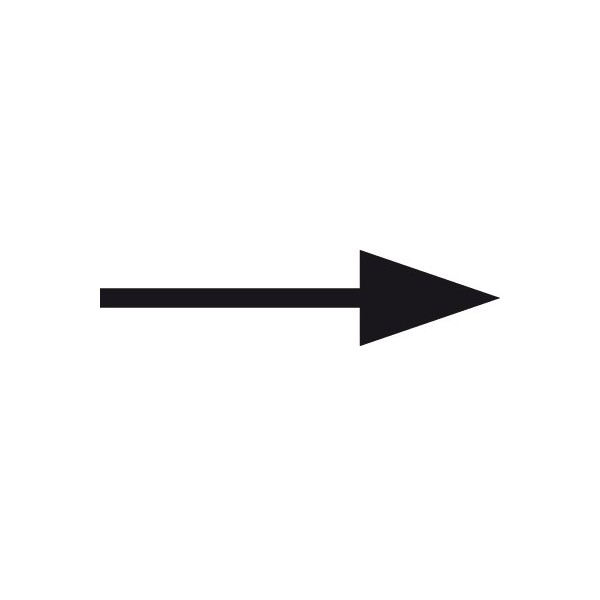
\includegraphics[scale=0.05]{images/image.jpg} \hfill        	
        	\includegraphics[scale=0.5]{images/jeu.PNG}
        	
			\end{figure}
			
			\item Suppression des lignes complètes, ligne malus, score et niveau
			\newline
			
			\begin{figure}[t]
        	
        	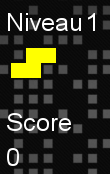
\includegraphics[scale=0.3]{images/score_niveau.PNG}
        	
			\end{figure}
			
		\end{enumerate}
		
		\begin{center}
			\underline{Calcul du score:}(25 * n + 100*(n-1))* niveau
			\newline
			\color{blue}
			\textit{n = nombre de lignes supprimées}
			
		\end{center}
		
		
	\end{frame}

\section{Pistes intelligence artificielle}
	
	

	\begin{frame}{La logique du bot}
	
		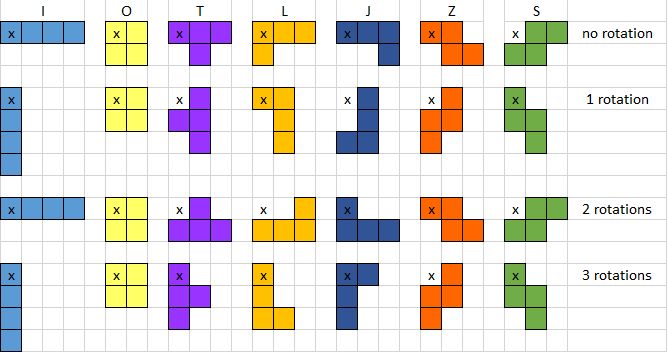
\includegraphics[scale=0.6]{images/rotation.png}

	\end{frame}
	
	

	\begin{frame}{Application de l'algorithme dans le logiciel}

		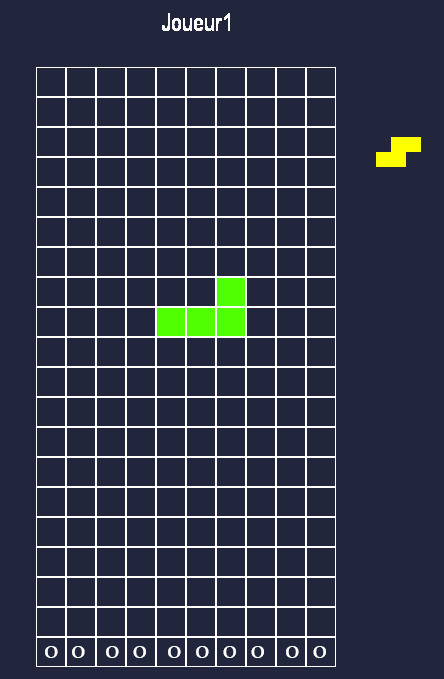
\includegraphics[scale=0.4]{images/Grille_0.png}\hfill
		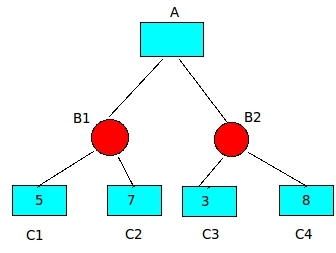
\includegraphics[scale=0.4]{images/minmax.jpg}

	\end{frame}
	
	
	
	\begin{frame}{Gestion de l'audio}
		\begin{center}
	
	
			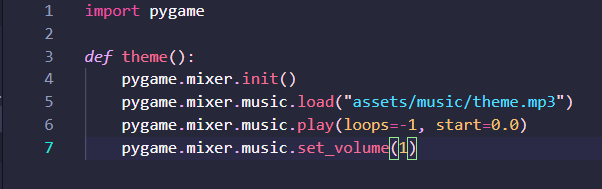
\includegraphics[width=250px]{images/audio.png}
			\\
			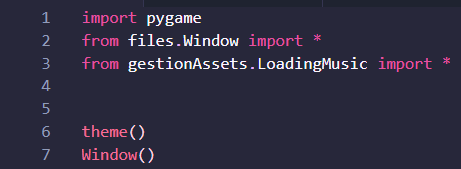
\includegraphics[width=150px]{images/main.png}

		\end{center}
	\end{frame}
	
\section{Explication piste réseau}

	
	\begin{frame}{Fonctionnement du réseau}

		\centering

		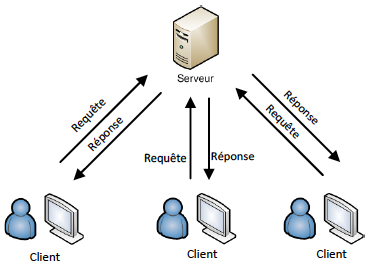
\includegraphics[width=120px]{images/schema.png}


		Lancement du serveur : \newline

		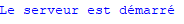
\includegraphics[width=120px]{images/serveur.png}
		\\
		Un client vient de se connecter au serveur : \newline
		\\
		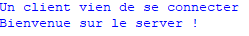
\includegraphics[width=150px]{images/client_conecter.png}

	\end{frame}
	
	
	
	\begin{frame}{Application du client et du serveur avec pygame}
		\centering
		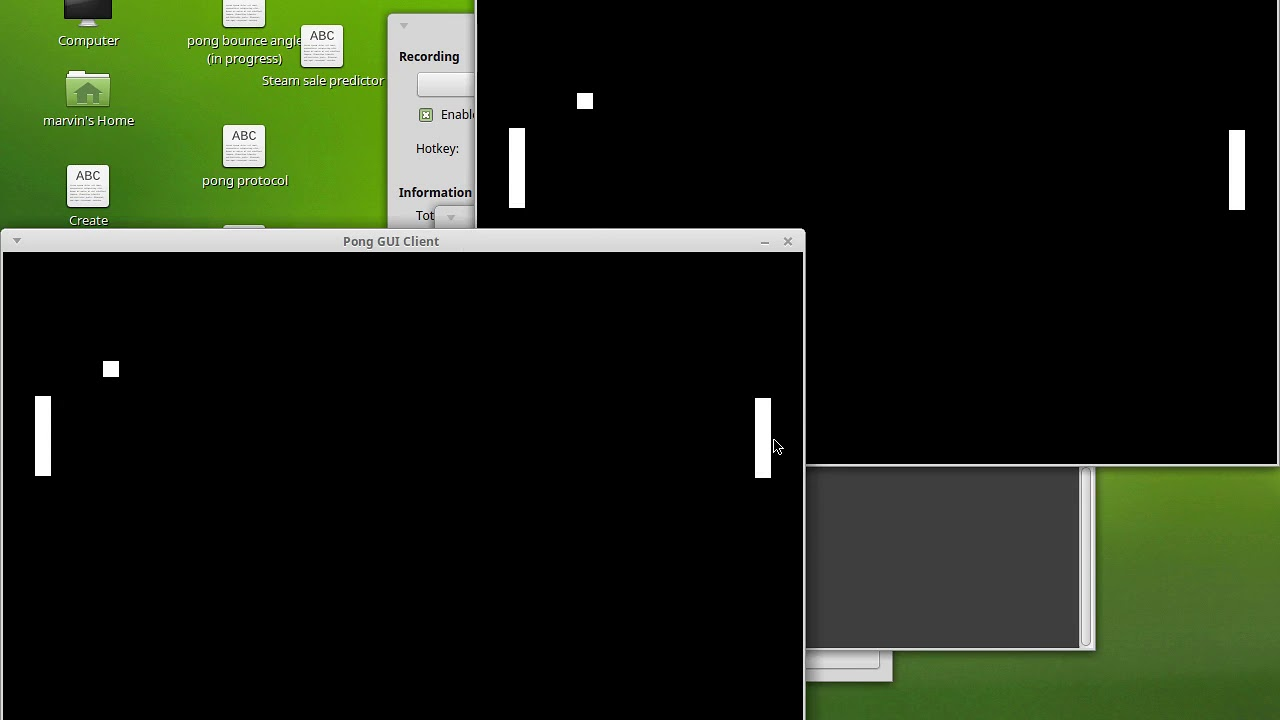
\includegraphics[width=300px]{images/multi_pygame.jpg}


	\end{frame}
	
\section{Démonstration}

	\begin{frame}
		 Début de la démonstration!
	\end{frame}
	
\section{Conclusion}

	\begin{frame}
		\begin{itemize}
			\item Un projet mené à bien malgré quelques bugs
			\newline
			
			\item Piste d'amélioration: un mode puzzle et de nouvelles fonctionnalités multijoueurs
		\end{itemize}
	\end{frame}
	
	\begin{frame}
		Merci de votre attention
	\end{frame}
\end{document}